\section{Objeto de estudio}
\label{sec:objeto-estudio}

El \textbf{objeto} es el YAML (o JSON) OpenAPI~3.x con el que un banco, un integrador o un
catálogo describe la API. Se puede parsear. Se puede poner al lado de un \ServiceDomain{}. No es
el banco, no es BIAN entero y no es el \textit{backend}.

BIAN entra como \textbf{referencia}: \textit{behaviors}, \textit{business objects}, control. El
consorcio también publica OpenAPI de muestra; esos YAML no son el objeto. El objeto es el
contrato \textbf{bancario} que se evalúa. El Anexo~F lo muestra con \textit{Payment Initiation}
sin convertirlo en el único caso.

Tres niveles, porque si se mezclan el score no se interpreta. La \Cref{fig:ontologia} y la
\Cref{tab:objeto-unidad-producto} los separan.

% Figura ontología conceptual — elaboración propia Grupo 10 (TikZ)
\begin{figure}[H]
  \centering
  \begin{tikzpicture}[
    font=\small\sffamily,
    box/.style={draw, rounded corners=2pt, align=center, minimum width=2.6cm,
                minimum height=0.85cm, fill=gray!8},
    ref/.style={box, fill=blue!8},
    prod/.style={box, fill=green!10},
    arr/.style={-{Stealth[length=2.2mm]}, thick, gray!70}
  ]
    \node[box] (sector) {Sector bancario\\APIs documentadas};
    \node[box, below=0.9cm of sector] (obj) {\textbf{Objeto:}\\contrato OpenAPI bancario};
    \node[ref, right=1.1cm of obj] (bian) {\textbf{Referencia:}\\\ServiceDomain{} BIAN};
    \node[box, below=0.9cm of obj] (ua) {\textbf{UA:}\\endpoint/schema $\leftrightarrow$\\ \Behavior{} / \BusinessObject{}};
    \node[prod, below=0.9cm of ua] (out) {\textbf{Producto:}\\S, E, C, \AlignmentScore{}};

    \draw[arr] (sector) -- (obj);
    \draw[arr] (obj) -- (ua);
    \draw[arr] (bian) -- (ua);
    \draw[arr] (ua) -- (out);
  \end{tikzpicture}
  \caption{Mapa conceptual del estudio: objeto, referencia, unidad de análisis y producto del
           modelo (elaboración propia).}
  \label{fig:ontologia}
\end{figure}


\begin{table}[H]
  \centering
  \caption{Objeto, unidad de análisis y producto del modelo}
  \label{tab:objeto-unidad-producto}
  \begin{tabular}{@{}p{0.28\textwidth}p{0.62\textwidth}@{}}
    \toprule
    \textbf{Concepto} & \textbf{En este estudio} \\
    \midrule
    \textbf{Objeto de estudio} & El contrato OpenAPI bancario completo (artefacto documental) \\
    \textbf{Unidad de análisis} &
    Elementos comparables dentro del \textit{pipeline}: endpoint/operation/schema $\leftrightarrow$
    \Behavior{} / \BusinessObject{} BIAN \\
    \textbf{Producto del modelo} & Scores S, E, C y \AlignmentScore{} por contrato evaluado \\
    \bottomrule
  \end{tabular}
\end{table}

El archivo es el objeto. Cada par endpoint--\Behavior{} o esquema--\BusinessObject{} es la
unidad. El \AlignmentScore{} y el nivel (Alta/Media/Baja/Nula) se reportan por instancia
\texttt{contrato} $\times$ \ServiceDomain{}.

Cada instancia se identifica de forma unívoca, p. ej.
\texttt{\{fuente\}\_\{service-domain\}\_\{version\}}, coherente con la adquisición de datos del
Capítulo~\ref{cap:metodologia} (§4.3).

\begin{table}[H]
  \centering
  \caption{Ejemplo genérico ilustrativo (sin caso piloto fijo)}
  \label{tab:ejemplo-generico}
  \begin{tabular}{@{}p{0.44\textwidth}p{0.44\textwidth}@{}}
    \toprule
    \textbf{Elemento OpenAPI (genérico)} & \textbf{Elemento BIAN de referencia (ilustrativo)} \\
    \midrule
    \texttt{POST /payment-orders} & \Behavior{} \texttt{Initiate} del dominio de pagos \\
    \texttt{GET /payment-orders/\{id\}} & \Behavior{} \texttt{Retrieve} \\
    Esquema \texttt{PaymentOrder} (propiedades \texttt{amount}, \texttt{currency}) &
    \BusinessObject{} \texttt{Payment} / \texttt{PaymentAmount} \\
    \bottomrule
  \end{tabular}
\end{table}


La tabla es \textbf{explicativa}: nombres ficticios para mostrar la unidad de análisis. El caso
ampliado de \textit{Payment Initiation} está en Anexo~F; el procedimiento aplica a cualquier
contrato OpenAPI bancario emparejado con un \ServiceDomain{} BIAN.
La \Cref{fig:objeto-unidad} resume objeto, unidad de análisis, producto del modelo y el ejemplo
genérico.

\begin{figure}[H]
  \centering
  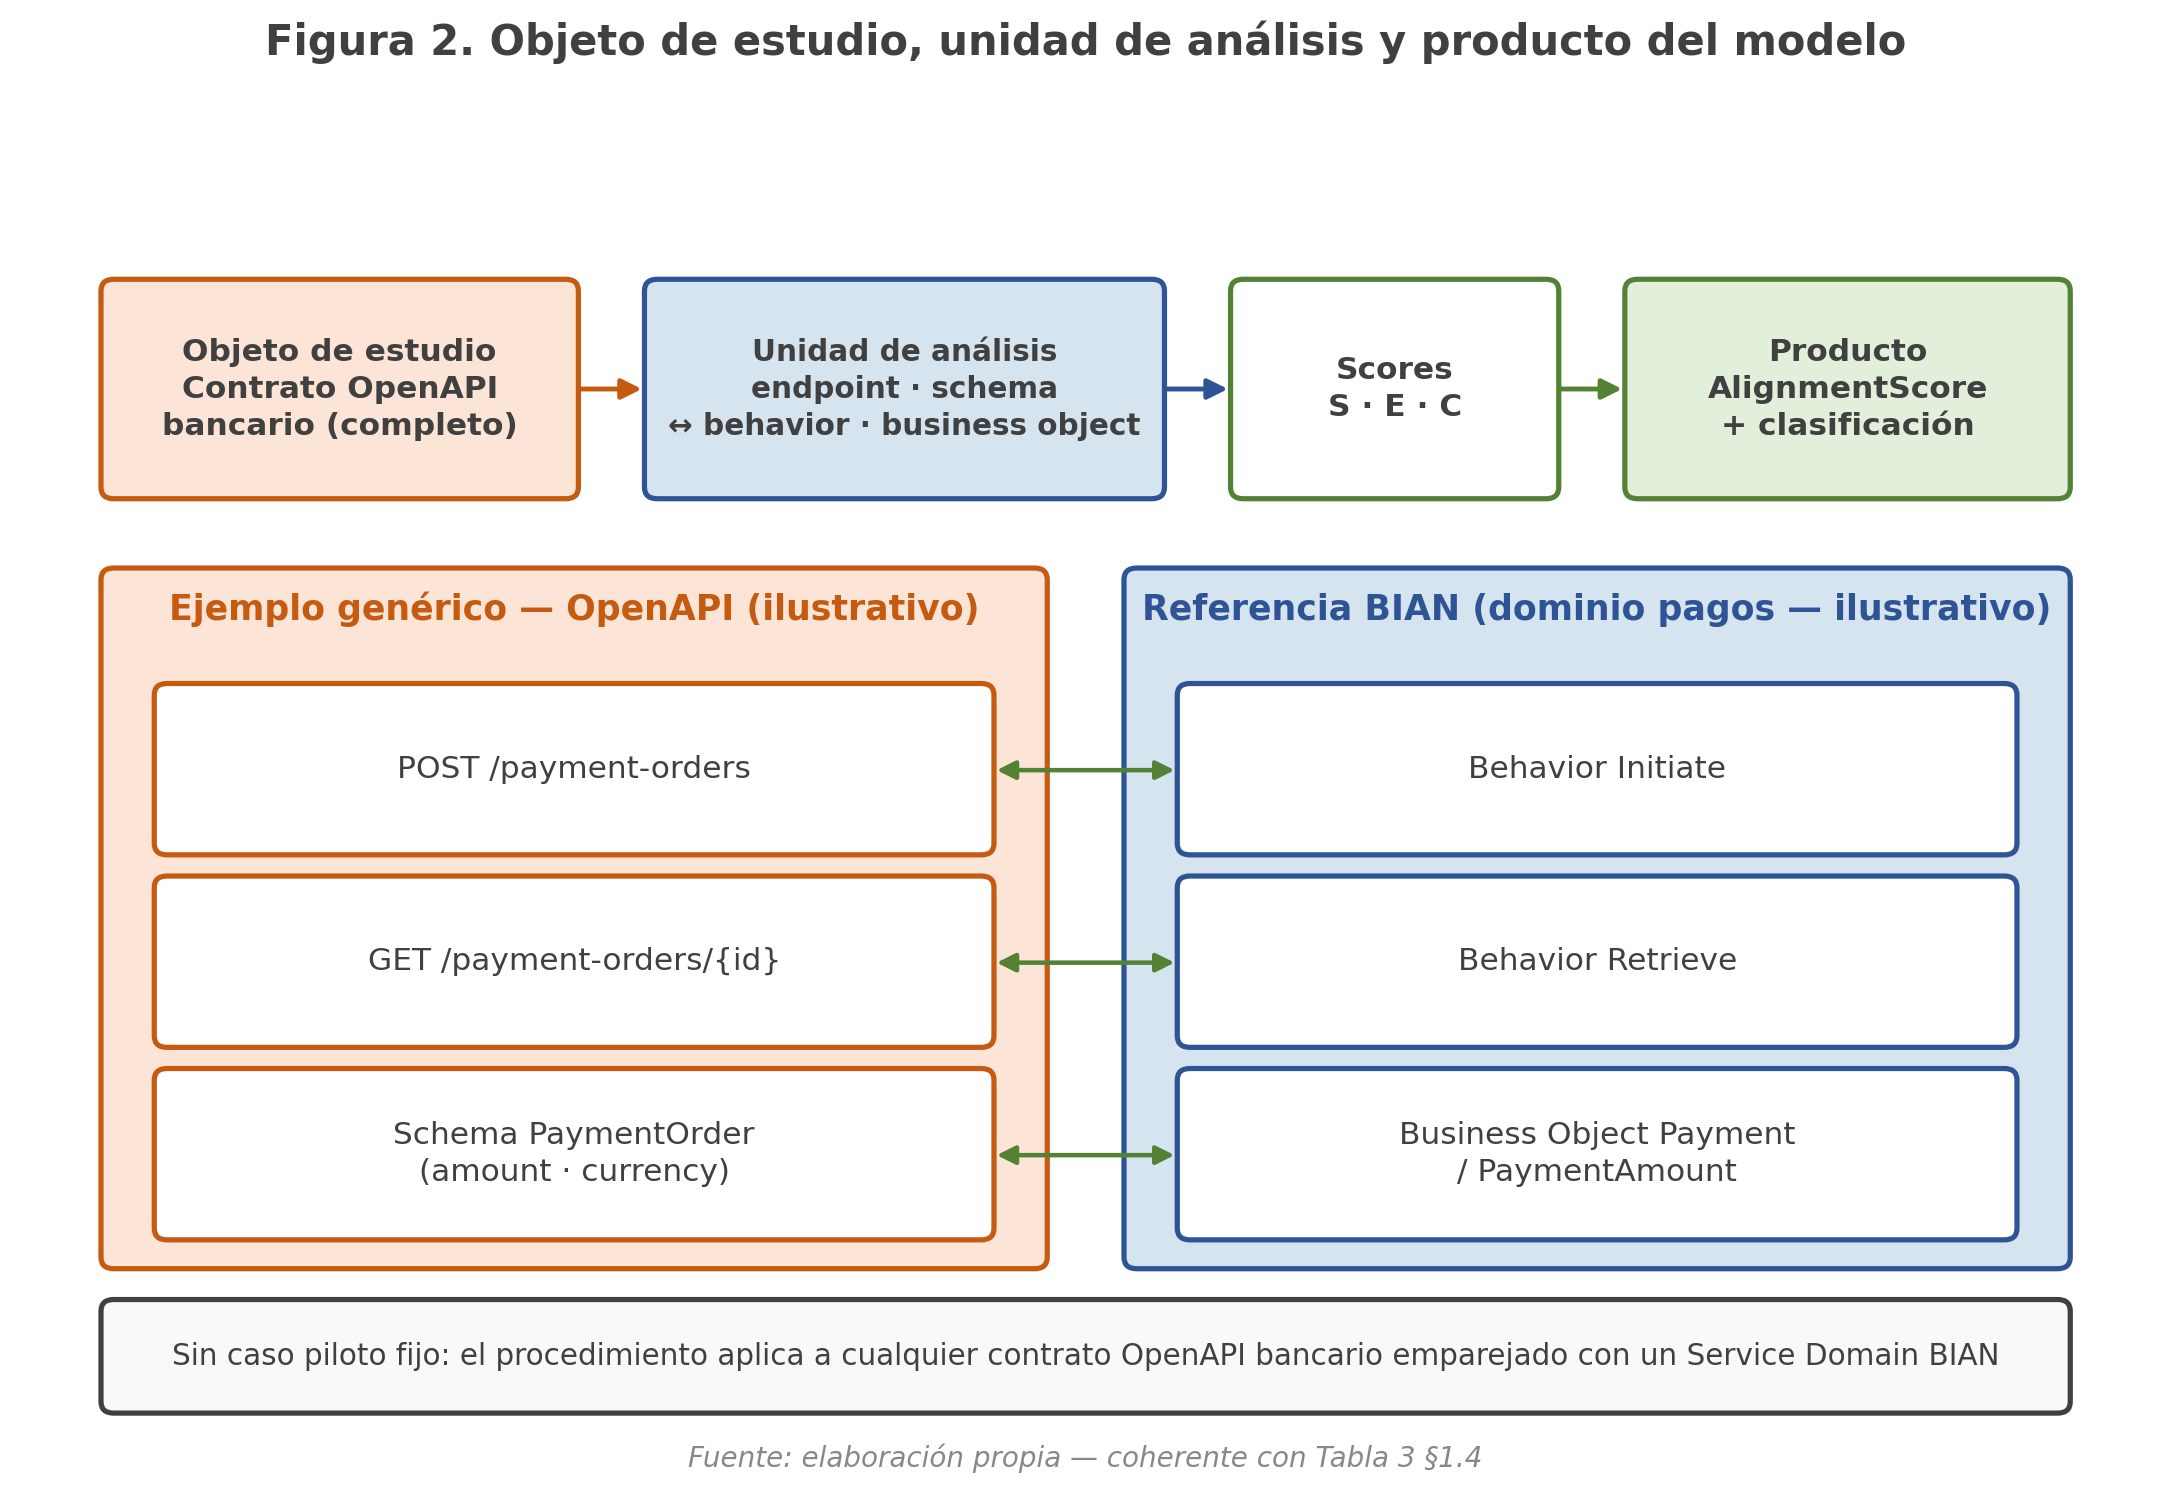
\includegraphics[width=0.92\textwidth]{Figura_02_Objeto_Unidad_Analisis}
  \caption{Objeto de estudio, unidad de análisis y producto (ejemplo genérico)}
  \label{fig:objeto-unidad}
\end{figure}

\subsection{Producto central: modelo de alineación}

Lo que la matriz pide como producto es el \textbf{modelo}, no un dashboard. Entrada: un contrato
y un SD emparejado. Salida:

\begin{table}[H]
  \centering
  \caption{Componentes del modelo de alineación}
  \label{tab:componentes-score}
  \begin{tabular}{@{}p{0.28\textwidth}p{0.62\textwidth}@{}}
    \toprule
    \textbf{Componente} & \textbf{Significado} \\
    \midrule
    \SemanticScore{} & Similitud de significado entre conceptos OpenAPI y BIAN \\
    \StructuralScore{} & Correspondencia de jerarquía y organización (REST $\leftrightarrow$ SD) \\
    \CoverageScore{} & Proporción de conceptos BIAN cubiertos por el contrato \\
    \bottomrule
  \end{tabular}
\end{table}

A partir de estos componentes se obtiene el \AlignmentScore{}:

\begin{quote}
  \AlignmentScore{} $= \alpha \cdot S + \beta \cdot E + \gamma \cdot C$, con $\alpha + \beta +
  \gamma = 1$
\end{quote}

La clasificación interpretativa del \textit{score} es: \textbf{Alta} ($\geq 0{,}80$),
\textbf{Media} (0,60--0,79), \textbf{Baja} (0,40--0,59) y \textbf{Nula} ($< 0{,}40$). Los umbrales
son \textbf{convención provisional del diseño} para este plan; su calibración empírica
permanece fuera del alcance (§1.6). Los scores S, E y C se calculan por unidad de análisis (par UA); el
\AlignmentScore{} y la clasificación se reportan por instancia contrato $\times$ \ServiceDomain{}.
La \Cref{fig:alignment-score} ilustra el cálculo del score de alineación.

\begin{figure}[H]
  \centering
  \figCapThree
  \caption{Cálculo del score de alineación: S, E, C $\rightarrow$ \AlignmentScore{}}
  \label{fig:alignment-score}
\end{figure}

Diseño, normalización, E, S, C y el score integrado: eso es Anexo~C y OE1--OE4
(Capítulo~\ref{cap:objetivos}).
